\documentclass[a4paper,12pt]{article} 
\usepackage[T2A]{fontenc}			
\usepackage[utf8]{inputenc}			
\usepackage[english,russian]{babel}	
\usepackage{amsmath,amsfonts,amssymb,amsthm,mathrsfs,mathtools} 
\usepackage{cancel}
\usepackage{multirow}
\usepackage[colorlinks, linkcolor = blue]{hyperref}
\usepackage{upgreek}\usepackage[left=2cm,right=2cm,top=2cm,bottom=3cm,bindingoffset=0cm]{geometry}
\usepackage{tikz}
\usepackage{graphicx}
\usepackage{subfig}
\usepackage{titletoc}
\usepackage{pgfplots}
\usepackage{xcolor}
\usepackage{wrapfig}
\usepackage{xfrac}
\usepackage{hhline}

\raggedbottom
\author{Дорогинин Д.В.\\
Группа Б02-825бф}
\title{Д4.3 Измерение толщины волоса.}
\date{}

%\begin{wrapfigure}{r}{0.5\textwidth}
%\begin{center}
%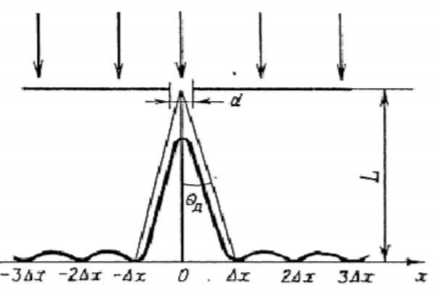
\includegraphics[width = 0.4\textwidth]{1.png}
%\end{center}
%\caption{}
%\end{wrapfigure}

%\begin{wrapfigure}{r}{0.5\textwidth}
%\begin{center}
%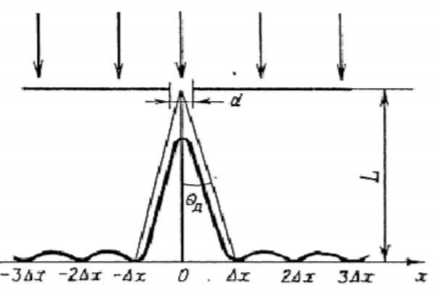
\includegraphics[width = 0.4\textwidth]{1.png}
%\end{center}
%\caption{}
%\end{wrapfigure}

\begin{document}
\maketitle
\textbf{Цель работы}: получить дифракционную картину на волосе и определить его толщину.


\textbf{В работе используются}: лазерная указка, волосы, картон, скотч, изолента, бумага, рулетка, линейка.

\begin{wrapfigure}[12]{r}{0.3\textwidth}
\begin{center}
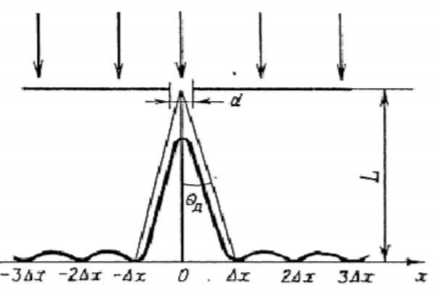
\includegraphics[width = 0.3\textwidth]{1.png}
\end{center}
\caption{Распределение интенсивности.}
\end{wrapfigure}
\section*{Теория}
Для света с длиной волны $\lambda$, нормально падающего на щель с толщиной $d \sim \lambda$, в приближении дифракции Фраунговера для координат минимумов выполняется соотношение
$$
d \sin \varphi_m = m\lambda,
$$
где $\sin \varphi_m$ -- угол отклонения, $m$ -- порядок минимума (Рис. 1). В приближении малых углов $\sin \varphi_m \approx \frac{x_m}{L}$, где $L$ -- расстояние от щели до экрана, $x_m$ -- расcтояние от нулевого максимума до минимума порядка $m$. Таким образом,
$$
x_m = \dfrac{m\lambda L}{d}.
$$
Отсюда видно, что расстояние $\Delta x$ между соседними минимумами постоянно, что даёт итоговую формулу для ширины щели:
\[
d = \dfrac{\lambda}{\Delta x}L. \tag{$\star$}
\]
\begin{figure}[h]
\begin{minipage}[h]{0.45\linewidth}
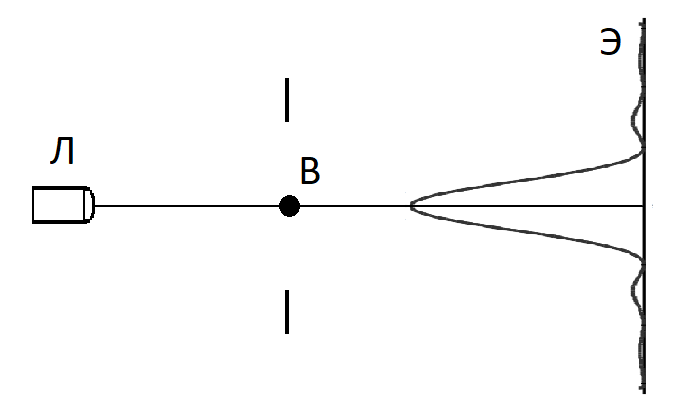
\includegraphics[scale=0.5]{2.png}
\centering
\end{minipage}
\hfill
\begin{minipage}[h]{0.45\linewidth}
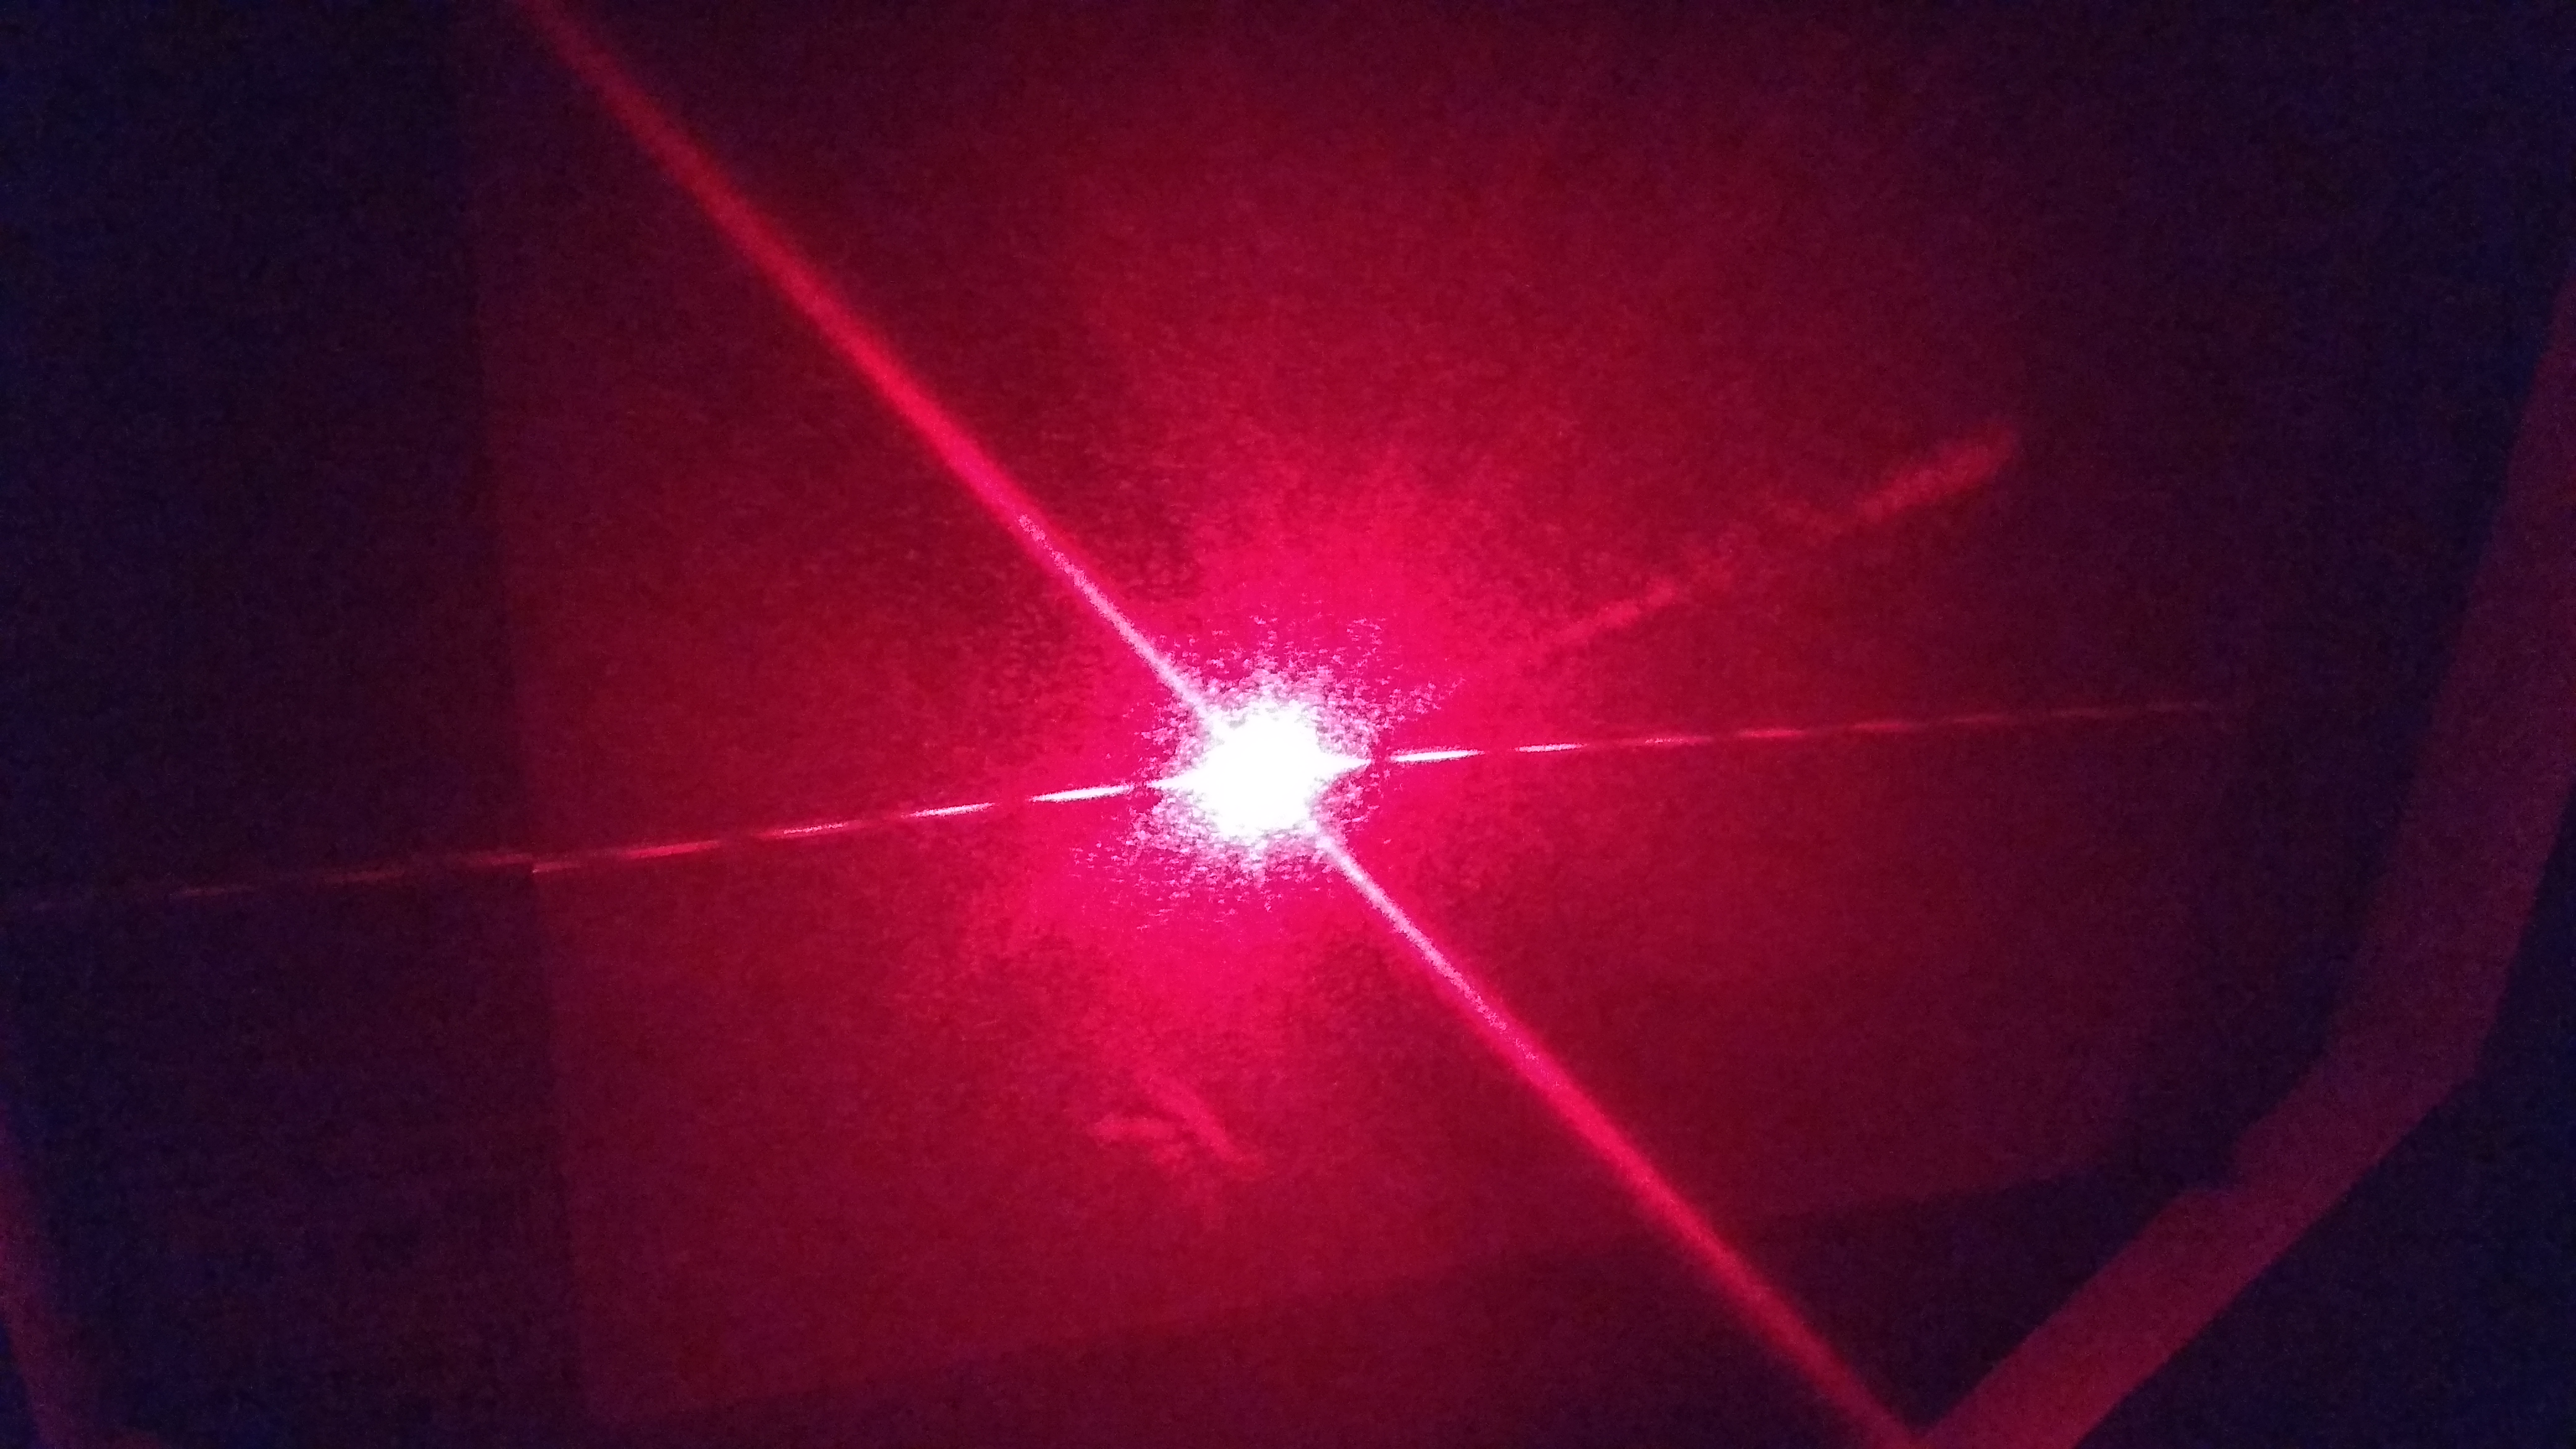
\includegraphics[scale=0.05]{4.jpg}
\centering
\end{minipage}
\centering
\caption{Схема установки (вид сверху) и пример дифракционной картины.}
\end{figure}\\
Схема установки представлена на Рис. 2. Эксперимент проводится в условиях минимальной освещённости. В куске картона вырезано прямоугольное отверстие, на нём закреплён натянутый волос В. Лазерная указка Л ($\lambda = 650~\text{нм}$) закрепляется изолентой на подставке во включённом состоянии. Свет от указки направляется на волос и падает перпендикулярно на экран Э, представляющий собой лист бумаги, закреплённый скотчем на раме. На экране наблюдается дифракционная картина (Рис. 2). Расстояние от экрана до волоса измеряется рулеткой. Для измерения расстояний $\Delta x$ между минимума на экране делаются штрихи ручкой в местах видимых минимумов, после чего измеряется расстояние $X$ между крайними видимыми минимумами и делится на количество промежутков.\\
Толщина волос измеряется для различных значений расстояния до экрана $L$, для этого подставка с указкой и картонка с волосом перемещаются на разные расстояния, экран при этом остаётся неподвижным. Так как свет падает на центральную часть волоса, изменение измеряемой толщины незаначительно при колебании высоты, так как волосы имеют одинаковый диаметр вдоль стрежня, не считая кончика, толщина которого не измерялась.

\begin{wrapfigure}[23]{r}{0.4\textwidth}
\begin{center}
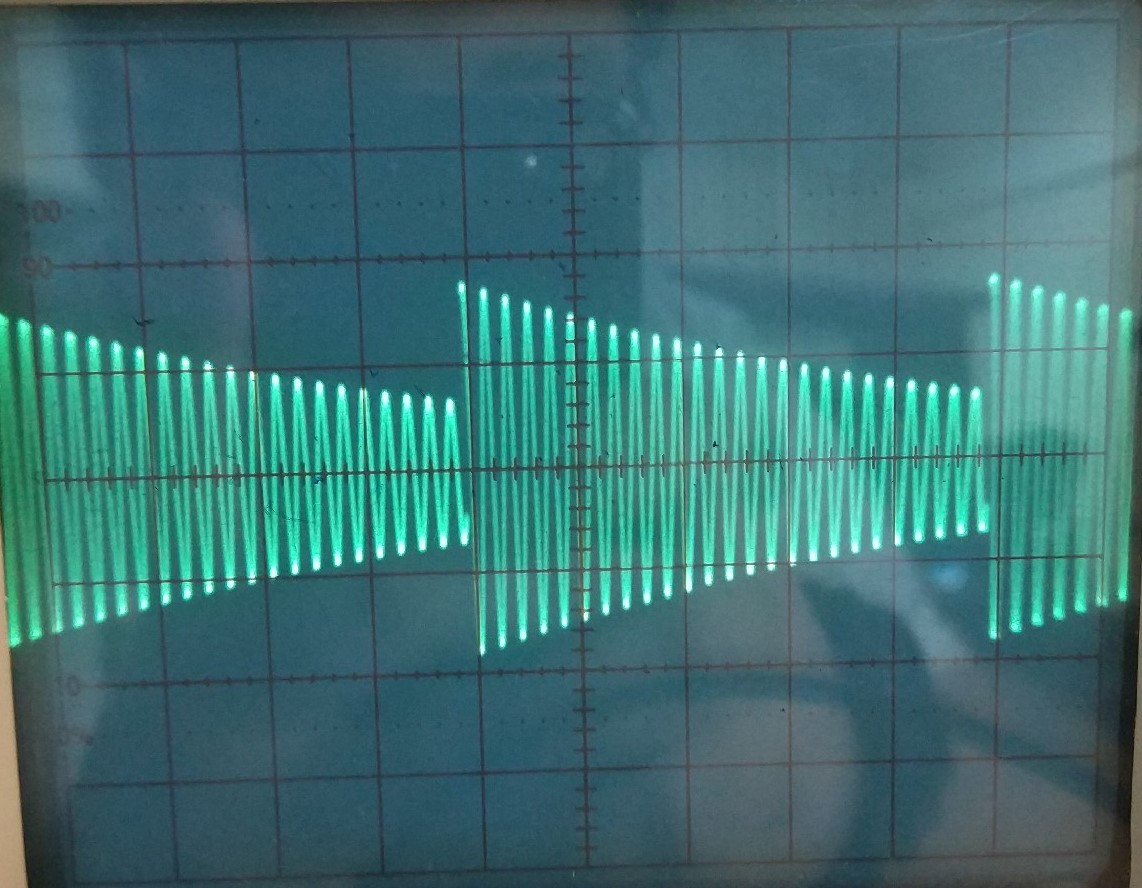
\includegraphics[width = 0.33\textwidth]{3.jpg}
\end{center}
\caption{Собранная установка.} 
\end{wrapfigure}
\section*{Ход работы}
Собираем установку согласно схеме (Рис. 3). В работе измеряются толщины трёх типов волос: человеческих, мужского и женского, и кошачьего. Результаты измерений представлены в Таблице 1. \\
Измерения не проводились для расстояний от волоса до экрана больших $150~\text{см}$, так как в этом случае наблюдается слишком мало дифракционный минимумов, что сказывается на погрешности, и для расстояний меньших $30~\text{см}$, так как в этом случае расстояние между минимумами становится слишком малым для точного подсчёта и нанесения штрихов.\\
Оценим, можно ли использовать приближение дифракции Фраунгофера, а именно соотношение
$$
\dfrac{d}{\sqrt{L\lambda}} \ll 1.
$$ 
Средняя толщина для волоса равна $70$ мкм, минимальное расстояние до экрана -- $30$ см, длина волны указки -- $650$ нм. Тогда 
$$ 
\dfrac{7\cdot 10^{-5}}{\sqrt{30\cdot 10^{-2} \cdot 650 \cdot 10^{-9}}} \approx 0.05 \ll 1 
$$ 
-- приближение выполняется, соответственно, для больших расстояний оно также выполняется.\\
Проверим, выполняется ли приближение малых углов. Для всех опытов оценим угол отклонения для наиболее отдалённого минимума как $\arctan{\frac{n \Delta x}{2 L}}$ -- для оценки считаем, минимумов было по $\frac{n}{2}$ по обе стороны от главного максимума. Максимальное значение угла, полученное таким образом, равно $0.085 \ll 1$ -- приближение малых углов также выполняется. Значит, формула $(\star)$ применима в условиях эксперимента. Рассчитаем с её помощью толщину волоса $d$ для каждого опыта, учитывая соотношение $\Delta x = \frac{X}{n}$.\\
Погрешность измерений $L$ принята $\sigma_L = 0.5~\text{см}$ из-за неточностей совпадения конца рулетки и экрана, делений рулетки и плоскости картонки, их неточной параллельности, а так же погрешности прямых измерений. Погрешность $X$ складывается из погрешности прямых измерений и неточности нанесения штрихов ровно на места минимумов, принята $\sigma_X = 0.2~\text{см}$. Количество промежутков $n$ считаем полученным с прогрешность в один ($\sigma_n = 1$) промежуток. Погрешность толщины волоса $d$ в отдельном опыте вычисляется по формуле
$$
\sigma_d = \sqrt{\left(\dfrac{\partial d}{\partial n}\right)^2 \sigma^2_n + \left(\dfrac{\partial d}{\partial X}\right)^2 \sigma^2_X + \left(\dfrac{\partial d}{\partial L}\right)^2 \sigma^2_L} = \lambda \sqrt{\dfrac{L^2}{X^2} \sigma^2_n + \dfrac{n^2 L^2}{X^4} \sigma^2_X + \dfrac{n^2}{X^2} \sigma^2_L}.
$$ 
\begin{table}[h]
\begin{tabular}{|c|c|c|c|c|c|c|c|c|c|c|c|c|c|}
\hline
\multicolumn{14}{|c|}{Мужской волос}                                                                             \\ \hline
$L$, см         & 30.0 & 40.0 & 50.0 & 60.0 & 70.0 & 80.0 & 90.0 & 100.0 & 110.0 & 120.0 & 130.0 & 140.0 & 150.0 \\ \hline
$n$             & 21   & 13   & 15   & 17   & 15   & 13   & 10   & 12    & 14    & 13    & 13    & 12    & 13    \\ \hline
$X$, см         & 4.9  & 4.0    & 5.8  & 7.8  & 7.7  & 7.6  & 6.6  & 8.7   & 11.1  & 11.1  & 12.2  & 12.6  & 13.7  \\ \hline
$d$, мкм        & 84   & 85   & 84   & 85   & 89   & 89   & 89   & 90    & 90    & 91    & 90    & 87    & 93    \\ \hline
$\sigma_d$, мкм & 5    & 8    & 6    & 6    & 6    & 7    & 9    & 8     & 7     & 7     & 7     & 7     & 7     \\ \hhline{|==============|}
\multicolumn{14}{|c|}{Женский волос}                                                                             \\ \hline
$L$, см         & 30.0 & 40.0 & 50.0 & 60.0 & 70.0 & 80.0 & 90.0 & 100.0 & 110.0 & 120.0 & 130.0 & 140.0 & 150.0 \\ \hline
$n$                 & 12   & 14   & 14   & 12   & 12   & 13   & 10   & 10    & 12    & 10    & 12    & 11    & 10    \\ \hline
$X$, см         & 3.8  & 5.5  & 6.7  & 7.2  & 8.4  & 9.9  & 8.9  & 9.4   & 12.2  & 11.6  & 14.8  & 14.4  & 14.1  \\ \hline
$d$, мкм        & 62   & 66   & 68   & 65   & 65   & 68   & 66   & 69    & 70    & 67    & 69    & 70    & 69    \\ \hline
$\sigma_d$, мкм & 6    & 5    & 5    & 6    & 6    & 5    & 7    & 7     & 6     & 7     & 6     & 6     & 7     \\ \hhline{|==============|}
\multicolumn{14}{|c|}{Кошачий волос}                                                                             \\ \hline
$L$, см         & 30.0 & 40.0 & 50.0 & 60.0 & 70.0 & 80.0 & 90.0 & 100.0 & 110.0 & 120.0 & 130.0 & 140.0 & 150.0 \\ \hline
$n$                 & 21   & 18   & 13   & 17   & 15   & 12   & 13   & 11    & 12    & 12    & 12    & 11    & 8     \\ \hline
$X$, см         & 5.1  & 5.6  & 5.4  & 8.0    & 8.4  & 7.8  & 9.4  & 8.8   & 11.2  & 11.5  & 12.1  & 11.8  & 9.9   \\ \hline
$d$, мкм        & 80   & 84   & 78   & 83   & 81   & 80   & 81   & 81    & 77    & 81    & 84    & 85    & 79    \\ \hline
$\sigma_d$, мкм & 5    & 6    & 7    & 5    & 6    & 7    & 6    & 8     & 7     & 7     & 7     & 8     & 10    \\ \hline
\end{tabular}
\centering
\caption{Результаты измерений.}
\end{table}\\
По результатам соответствующих опытов определим итоговую толщину каждого волоса $d_0$, которая вычисляется как среднее арифметической полученных значений:
$$
d_0 = \dfrac{\sum d}{N},
$$
где суммируются все полученные длины волос, $N = 13$ -- количество опытов. Её погрешность складывается из случайной ошибки $\sigma_{\text{случ}}$ и систематической погрешности $\sigma_{\text{сист}}$. Случайную ошибку вычисляем как
$$
\sigma_{\text{случ}} = \sqrt{\dfrac{\sum(d_0 - d)^2}{N(N-1)}},
$$
где суммирование ведётся по всем опытам. Систематическую погрешность рассчитаем как  
$$
\sigma_{\text{сист}} = \sqrt{\sum \left( \dfrac{\partial d_0}{\partial d}\right)^2 \sigma^2_d} = \dfrac{\sqrt{\sum \sigma^2_d}}{N},
$$
где суммирование, опять же, ведётся по всем соответсвующим опытам.\\
Итоговые значения толщин $d_0$ представлены в Таблице 2. Обратим внимание, что представленный способ измерения оказался достаточно точным -- относительная погрешность не превышает $3.5\%$. Полученные толщины лежат в диапазоне возможных для волос -- $17 \div 180$ мкм.
\begin{table}[h]
\begin{tabular}{|c|c|c|}
\hline
Волос   & $d_0$, мкм & $\sigma_{d_0}$, мкм \\ \hline
Мужской & 88       & 3                   \\ \hline
Женский & 67       & 2                 \\ \hline
Кошачий & 81       & 2                 \\ \hline
\end{tabular}
\centering
\caption{Итоговые значение толщин $d_0$.}
\end{table}
\end{document}